\section{Implementacja agentów}
\label{sec:implementacjaAgentow} 

\par Agenci stanowią główny decyzyjny systemu. To w nich znajduje się logika odpowiedzialna za podejmowanie decyzji, reagowanie na zmiany i obsługę komunikatów nadawanych przez innych. Podstawowymi założeniami systemów agentowych jest ich autonomiczność, zdolność do komunikacji oraz możliwość postrzegania i wpływania na środowisko. Aby spełnić te wymagania koniecznym były zapewnienie pewnych mechanizmów.

\par Podstawą działania agentów, jest ich umiejętność do postrzegania otoczenia. Odbywa się to przy użyciu \texttt{IEnvironmentSignal}. Każdy agent w systemie definiuje, jakie sygnały z otoczenia potrafi obsłużyć. Następnie serwisy działające w ramach aplikacji, w której żyje nasz agent przekazują mu te sygnały. Trafiają one do specjalnej kolejki, skąd zostaną później obsłużone.

\par Zdolność do działania przejawia się poprzez dostęp do funkcji sprzętowych z poziomu aplikacji. Dla przykładu, \emph{Navigation Agent} potrafi wykorzystać \texttt{INavigationService}, aby ten wyświetlił patrolowi drogę do wyznaczonego celu.

\par Komunikacja między agentami odbywa się przy wykorzystaniu \emph{Message Bus}a., opisanego w podrozdziale \ref{sec:infrastrukturaKomunikacyjna}. Wszystkie wiadomości spełniają interfejs \texttt{IMessage}, a agenci definiują które ich typy są w stanie obsłużyć. Oczywiście sama możliwość wysłania komunikatu, nie rozwiązuje wszystkich problemów w dialogu, dlatego też zostały zaimplementowane dwa dodatkowe mechanizmy rozszerzające bazowe możliwości.

\par Pierwszym z nich jest możliwość odpytania\english{Ask} innego agenta i oczekiwania na odpowiedź. Jest to niezbędny mechanizm, podczas podejmowania decyzji wymagających danych, których dany agent nie posiada.

\par Drugim wysyłanie wiadomości wymagających potwierdzenia odbioru\english{Requiring Acknowledgment}. Dla nich powstał specjalny interfejs \texttt{IMessageWithAcknowledgeRequired} rozszerzający \texttt{IMessage}. Mechanizm ten jest wykorzystywany podczas wysyłania rozkazów przez \emph{HQ Agent}, aby mieć pewność ich akceptacji.

\par Podstawowe założenia agenta w systemie definiuje interfejs \texttt{IAgent}. Określa on konieczność zdefiniowania akceptowanych typów sygnałów środowiskowych i akceptowanych typów wiadomości. Klasa \texttt{AgentBase} jest bazową implementacją rozszerzającą tę definicję o wspomniane wcześniej mechanizmy potwierdzania wiadomości i odpytywania innych agentów.

\par Agenci spełniają dodatkowo \texttt{IHostedService}, co pozwala na uruchomienie ich, jako długo działające\english{Long Running} programy\cite{BACKGROUND_TASKS_WITH_HOSTED_SERVICES}. Ich działanie jest w pełni asynchroniczne. Dzięki zastosowaniu mechanizmu dostępu warunkowego, w postaci \texttt{AsyncReaderWriterLock} pochodzącego z biblioteki \emph{AsyncEx}\cite{STEPHEN_CLEARY_ASYNCEX_GITHUB}, mogą oni odczytywać wiadomości, które trafiły do kolejek. Cykl działania agenta przedstawia rysunek \ref{fig:agentsAgentCycle}.

\begin{figure}
    \centering
    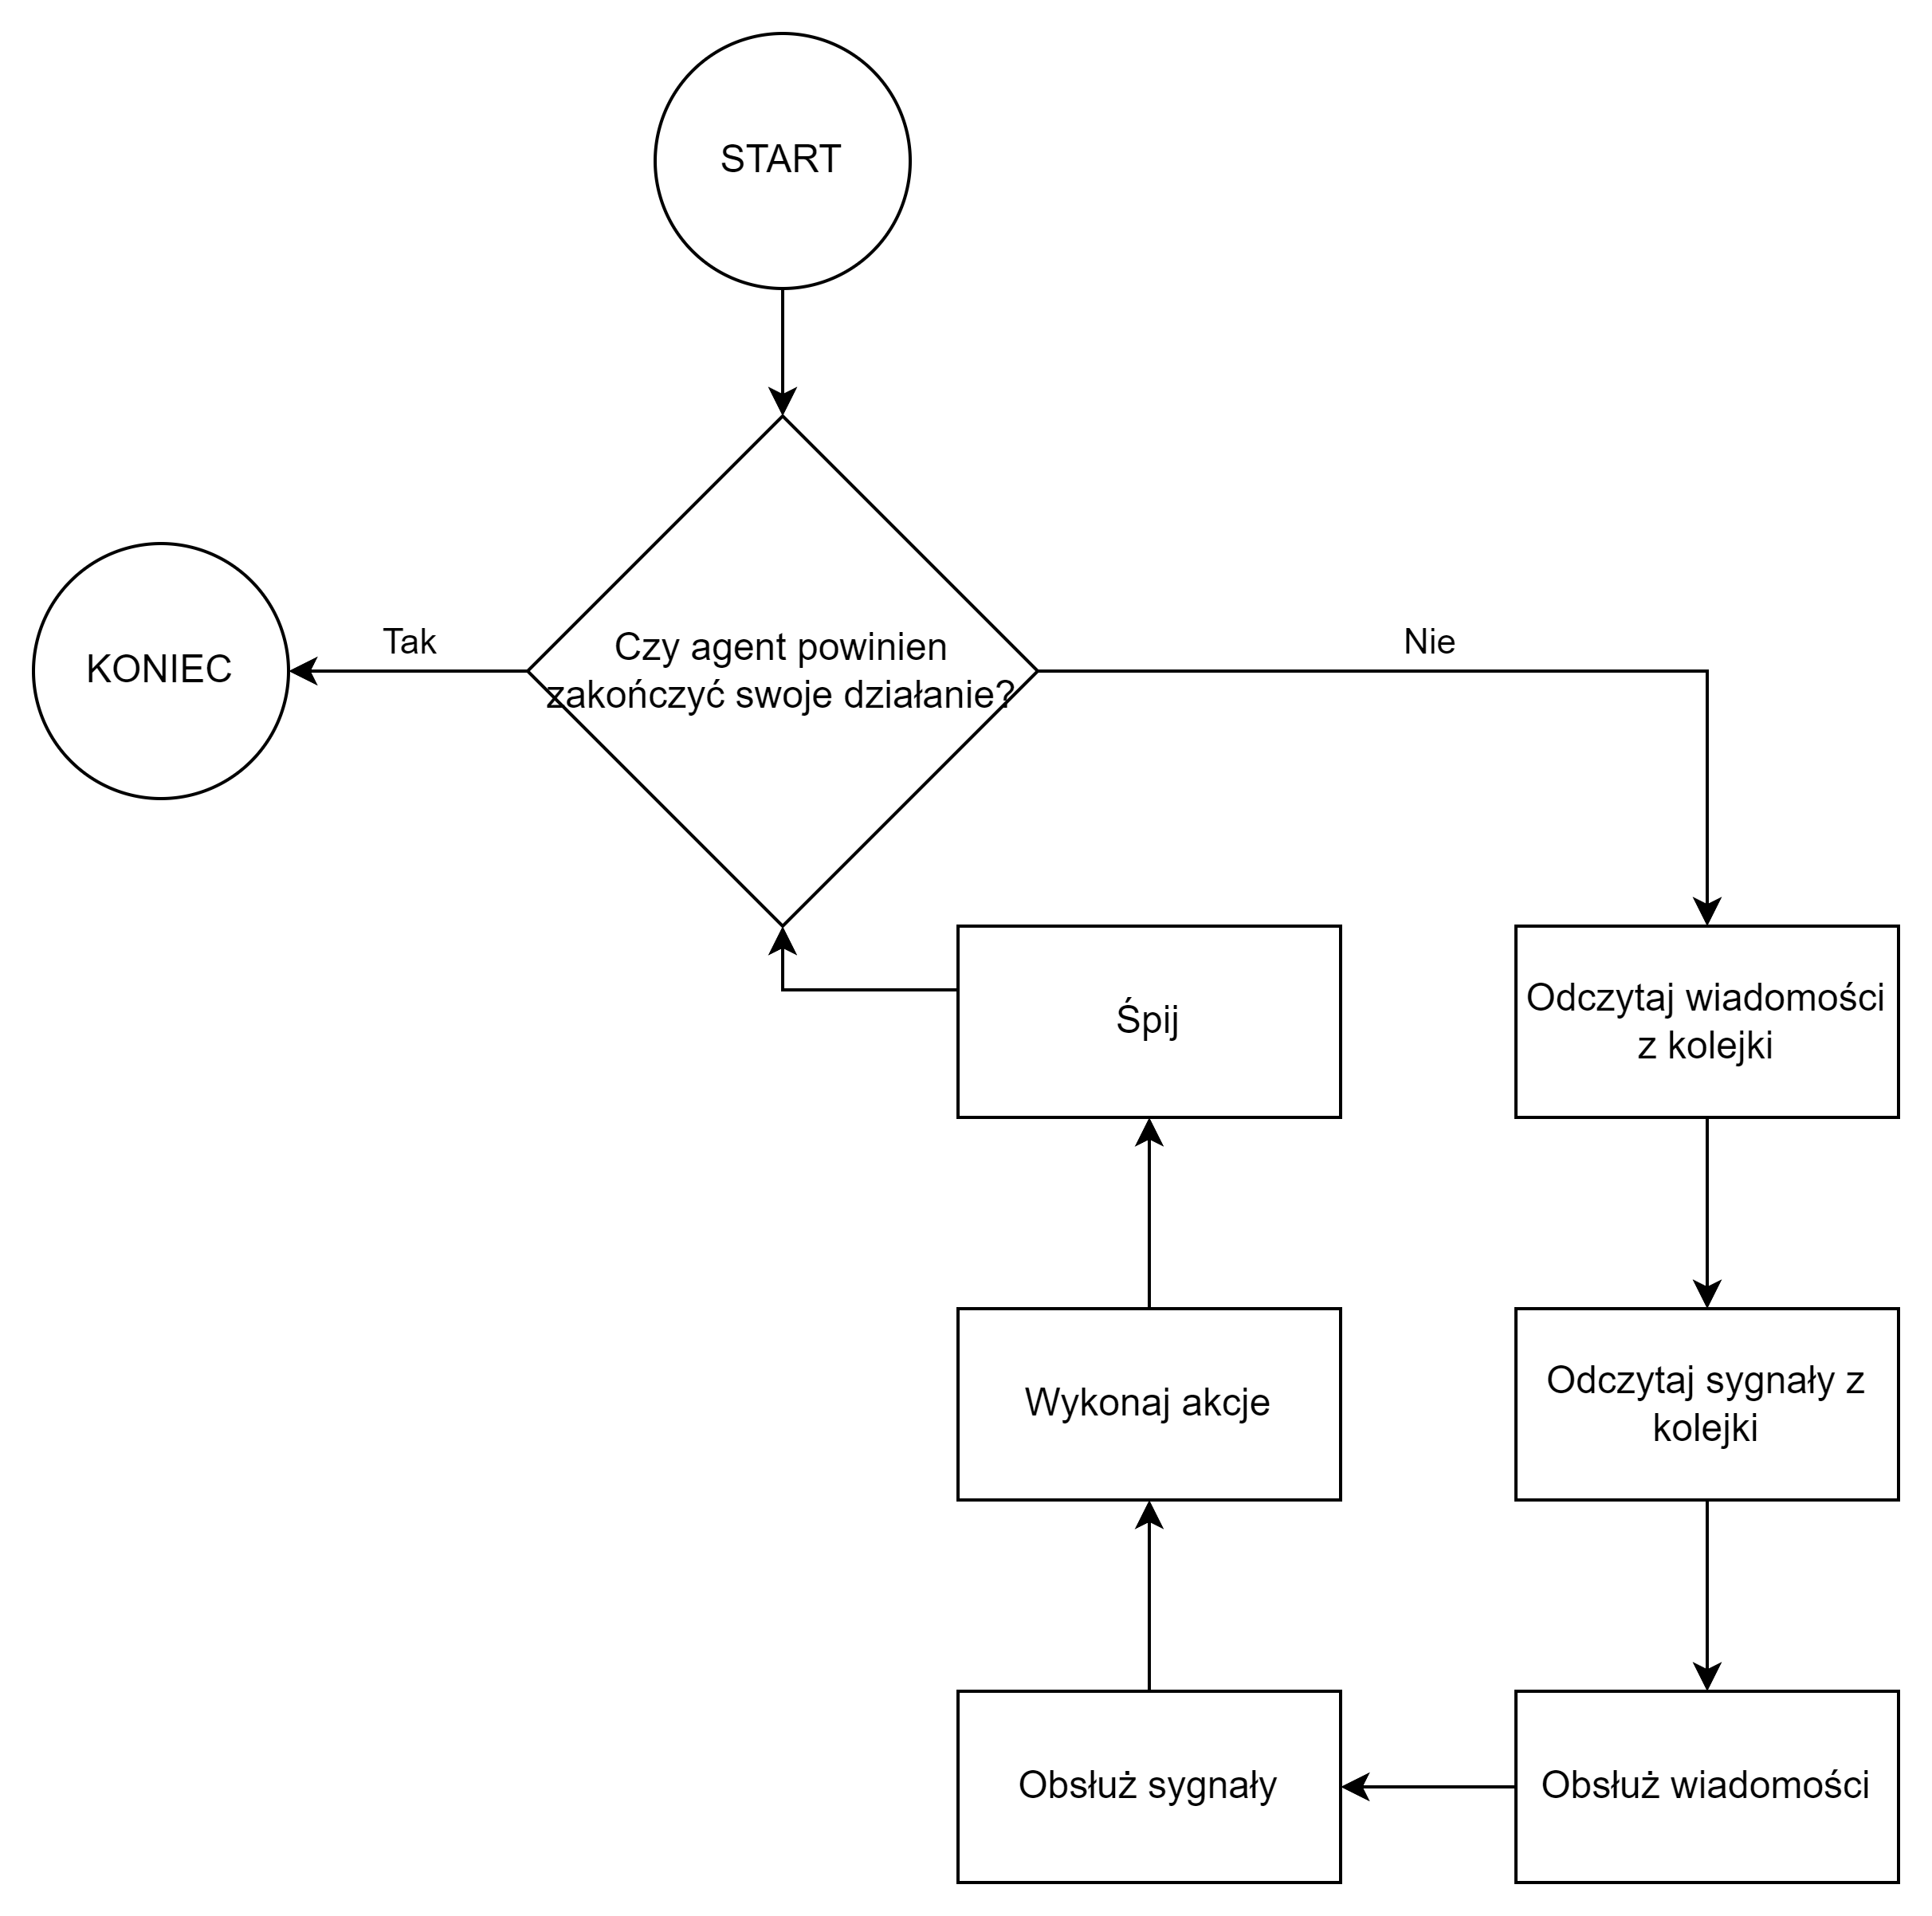
\includegraphics[width=\linewidth]{Agents - Agent Cycle}
    \caption{Cykl działania agenta}
    \label{fig:agentsAgentCycle}
    \source{Opracowanie Własne}
\end{figure}

\par Aby spełnić założenia systemu, ważnym było dokładne określenie wymiany wiadomości między agentami. Tabela \ref{tab:agentsMessagesSenderReceiver} pokazuje relację między typem wiadomości, a jej odbiorcą i nadawcą.

\begin{table}
    \centering
    \begin{tabular}{|c|c|c|} 
     \hline
     Rodzaj wiadomości & Nadawca & Odbiorca \\
     \hline
     \hline
     AskPositionMessage & Patrol Agent & Navigation Agent \\ 
     \hline
     CurrentLocationMessage & Navigation Agent & Patrol Agent \\ 
     \hline
     CurrentLocationMessage & Patrol Agent & HQ Agent \\ 
     \hline
     DestinationReachedMessage & Navigation Agent & Patrol Agent \\ 
     \hline
     GunFiredMessage & Gun Agent & Patrol Agent \\ 
     \hline
     GunFiredMessage & Patrol Agent & HQ Agent \\ 
     \hline
     IncidentInvestigationStartedMessage & Patrol Agent & HQ Agent \\ 
     \hline
     IncidentResolvedMessage & Patrol Agent & HQ Agent \\ 
     \hline
     JoinedShootingMessage & Patrol Agent & HQ Agent \\ 
     \hline
     NavigateToMessage & Patrol Agent & Navigation Agent \\ 
     \hline
     PatrolOfflineMessage & Patrol Agent & HQ Agent \\ 
     \hline
     PatrolOnlineMessage & Patrol Agent & HQ Agent \\ 
     \hline
     PatrolStatusChangedMessage & Patrol Agent & HQ Agent \\ 
     \hline
     ShowDistrictMessage & Patrol Agent & Navigation Agent \\ 
     \hline
     HandleIncidentOrderMessage & HQ Agent & Patrol Agent \\ 
     \hline
     PatrolDistrictOrderMessage & HQ Agent & Patrol Agent \\ 
     \hline
     SupportShootingOrderMessage & HQ Agent & Patrol Agent \\ 
     \hline
    \end{tabular}
    \caption{Tabela relacji wiadomości, nadawcy i odbiorcy}
    \label{tab:agentsMessagesSenderReceiver}
\end{table}

\par Zdefiniowane został również sygnały środowiskowe, służące agentom do obserwowania zmian w ich otoczeniu. Przedstawia je tabela \ref{tab:agentsEnvironmentSignals}.

\begin{table}
    \centering
    \begin{tabular}{|c|c|} 
     \hline
     Rodzaj sygnału & Agent \\
     \hline
     \hline
     DestinationReachedSignal & Navigation Agent \\ 
     \hline
     GunFiredSignal & Gun Agent \\ 
     \hline
     IncidentAlreadyOverSignal & Patrol Agent \\ 
     \hline
     IncidentResolvedSignal & Patrol Agent \\ 
     \hline
     PositionChangedSignal & Navigation Agent \\ 
     \hline
    \end{tabular}
    \caption{Tabela sygnałów środowiskowych wraz z ich odbiorcami}
    \label{tab:agentsEnvironmentSignals}
\end{table}

\par Aby komunikacja mogła nastąpić pomiędzy agentami, koniecznym jest ich odpowiednia konfiguracja. W szczególności dotyczy to patroli, które muszą wiedzieć, z jakich elementów się składają. W tym celu powstał interfejs \texttt{IPatrolInfoService}, który zapewnia informacje o identyfikatorach \emph{Patrol Agent}, \emph{Navigation Agent} i \emph{Gun Agent} oraz identyfikator patrolu, jako całości. Dokładniejszy opisz konfiguracji został omówiony w podrozdziale \ref{sec:konfiguracja}.